% Compilation : XeLaTeX, deux passes (ou latexmk -xelatex).
% Les cinq images du dossier figures/ sont nécessaires.
% Version concise : exactement sept diapositives, sans annexe.
\documentclass[aspectratio=169,11pt]{beamer}
\geometry{paperwidth=320mm,paperheight=180mm}
\usepackage{fontspec,unicode-math}
\setsansfont{Latin Modern Sans}
\setmainfont{Latin Modern Sans}
\setmathfont{Latin Modern Math}
\usepackage{graphicx,booktabs,array,tabularx}
\usefonttheme{professionalfonts}
\definecolor{navy}{HTML}{183047}
\definecolor{teal}{HTML}{007F83}
\definecolor{muted}{HTML}{63717B}
\definecolor{rulegray}{HTML}{DDE3E7}
\setbeamercolor{normal text}{fg=navy,bg=white}
\setbeamercolor{structure}{fg=teal}
\setbeamercolor{frametitle}{fg=navy,bg=white}
\setbeamercolor{footline}{fg=muted,bg=white}
\setbeamersize{text margin left=14mm,text margin right=14mm}
\setbeamerfont{normal text}{size=\fontsize{22}{28}}
\setbeamerfont{frametitle}{size=\fontsize{31}{36},series=\bfseries}
\setbeamerfont{itemize/enumerate body}{size=\fontsize{22}{28}}
\setbeamertemplate{navigation symbols}{}
\setbeamertemplate{itemize item}{\color{teal}\small\textbullet}
\setbeamertemplate{frametitle}{%
  \par\vspace{5mm}\insertframetitle\par\vspace{3mm}%
  {\color{rulegray}\hrule height .6pt}\par\vspace{4mm}}
\newcommand{\framesource}{}
\newcommand{\src}[1]{\gdef\framesource{#1}}
\setbeamertemplate{footline}{%
  \begin{beamercolorbox}[wd=\paperwidth,ht=5mm,dp=3mm,leftskip=14mm,rightskip=14mm]{footline}
    \fontsize{10}{12}\selectfont\framesource\hfill\insertframenumber/7
  \end{beamercolorbox}}
\setlength{\parskip}{2.5mm}
\newcommand{\key}[1]{{\color{teal}\bfseries #1}}
\newcommand{\smalltxt}{\fontsize{19}{24}\selectfont}
\newcommand{\captiontxt}{\fontsize{17}{21}\selectfont}
\newcommand{\lightline}{\par\vspace{7mm}{\color{rulegray}\hrule height .5pt}\par\vspace{9mm}}
\newcommand{\bignum}[1]{{\fontsize{34}{39}\selectfont\color{teal}\bfseries #1}}
\graphicspath{{figures/}}
\hypersetup{
  pdftitle={XYZ-IBD : présentation en sept diapositives},
  pdfauthor={Mattis BORDERIES},
  colorlinks=true,urlcolor=teal
}

\begin{document}
\usebeamerfont{normal text}

% 1. Introduction : figures 1 et 4 de l'article.
\begin{frame}{XYZ-IBD : perception industrielle}
\src{Huang et al., XYZ-IBD, introduction et figures 1 et 4. Présentation : Mattis BORDERIES.}
\textbf{Dévracage robotique : estimer la pose 6D de pièces empilées.}

\par\vspace{3mm}
\begin{columns}[T,onlytextwidth]
\begin{column}{.48\textwidth}
\begin{minipage}[c][66mm][c]{\linewidth}
\centering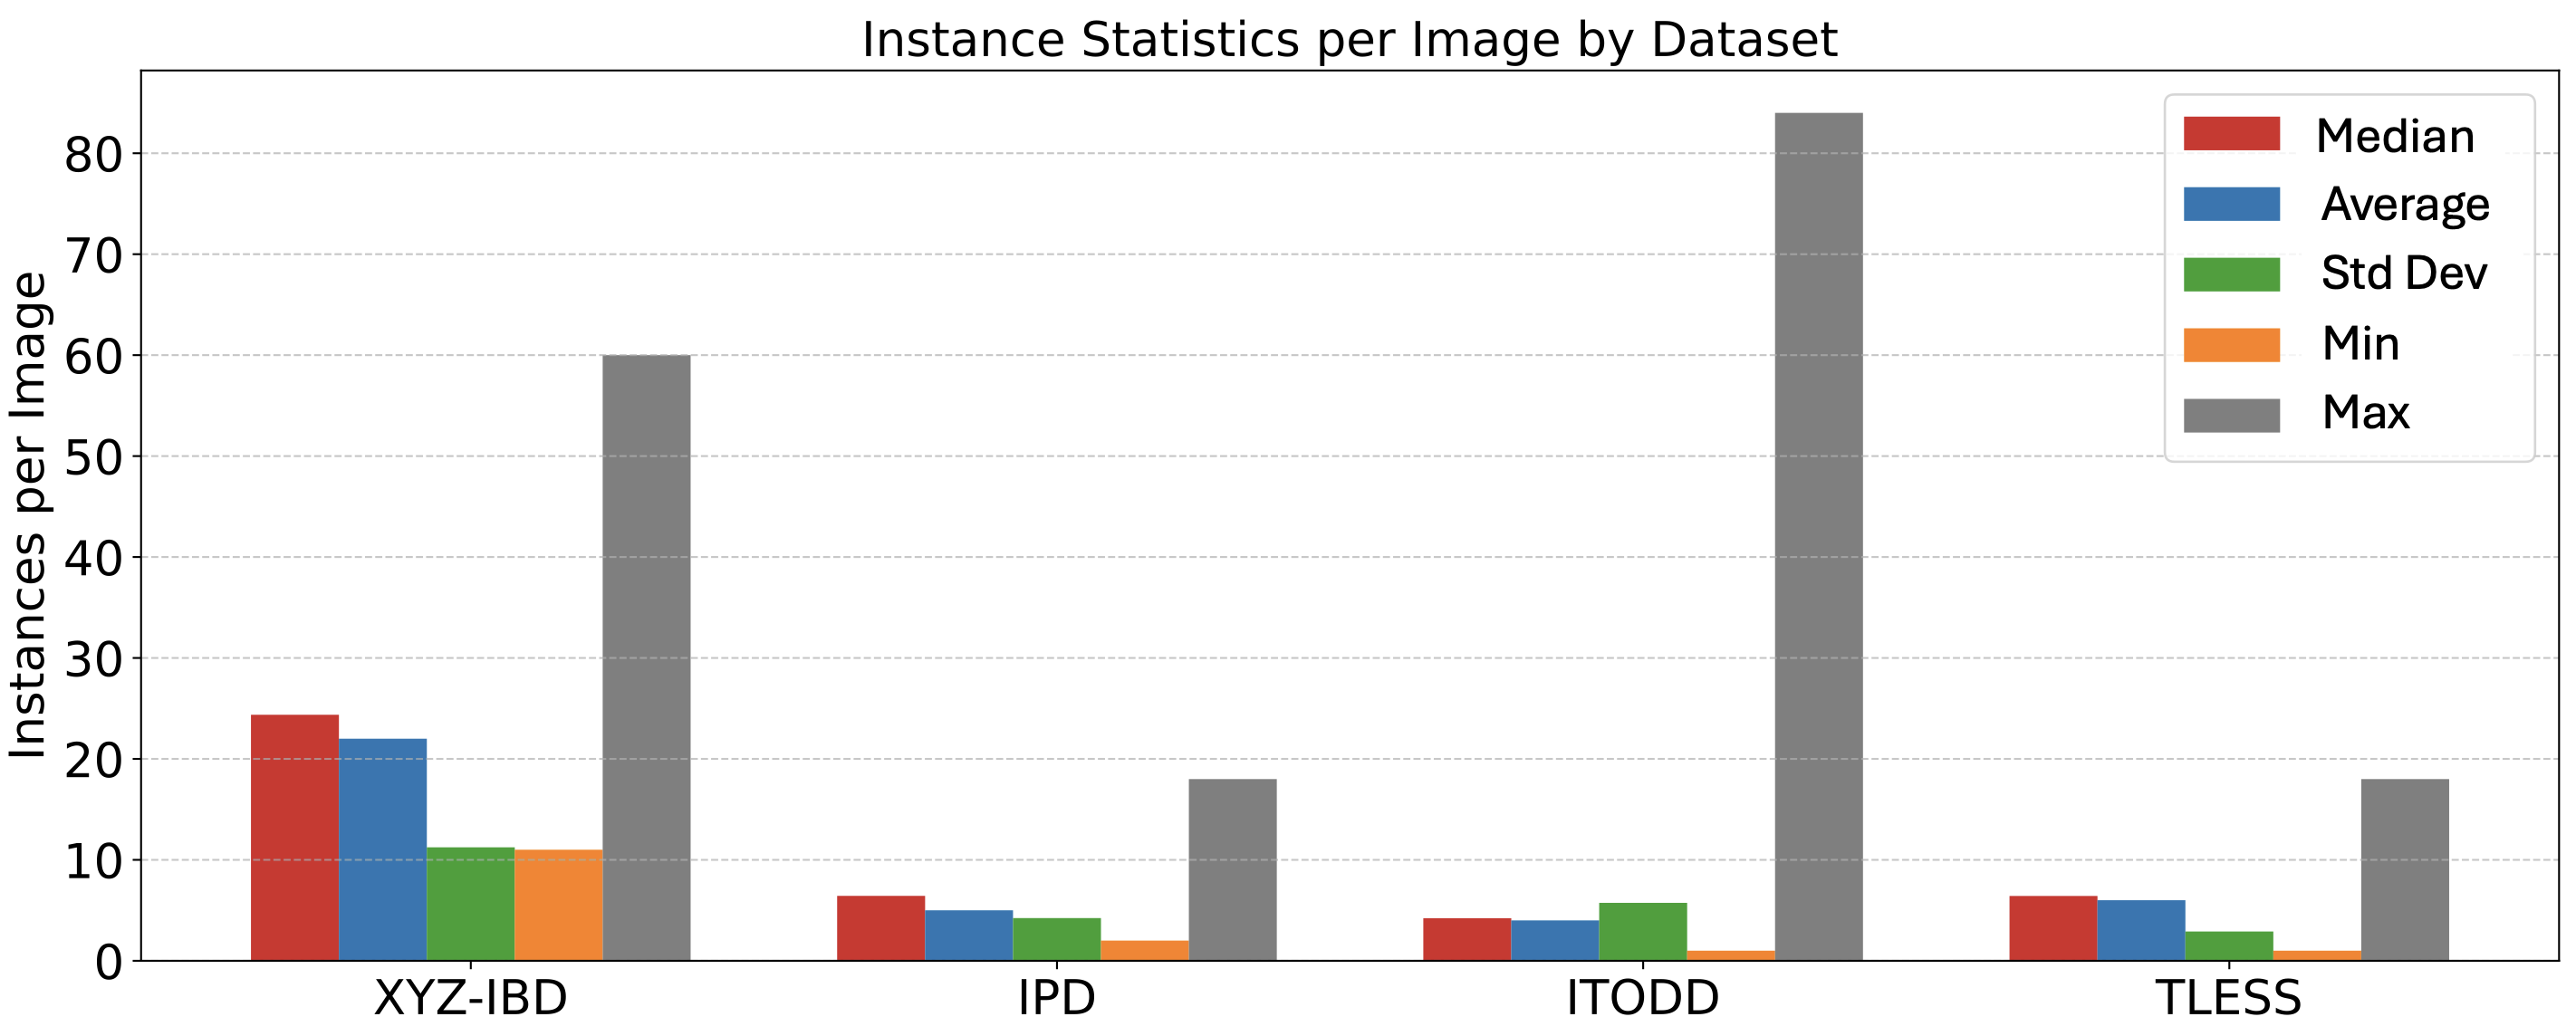
\includegraphics[width=\linewidth]{dataset_comparaison.png}
\end{minipage}
\par\centering\smalltxt\textbf{Forte densité d'instances}
\end{column}
\begin{column}{.48\textwidth}
\begin{minipage}[c][66mm][c]{\linewidth}
\centering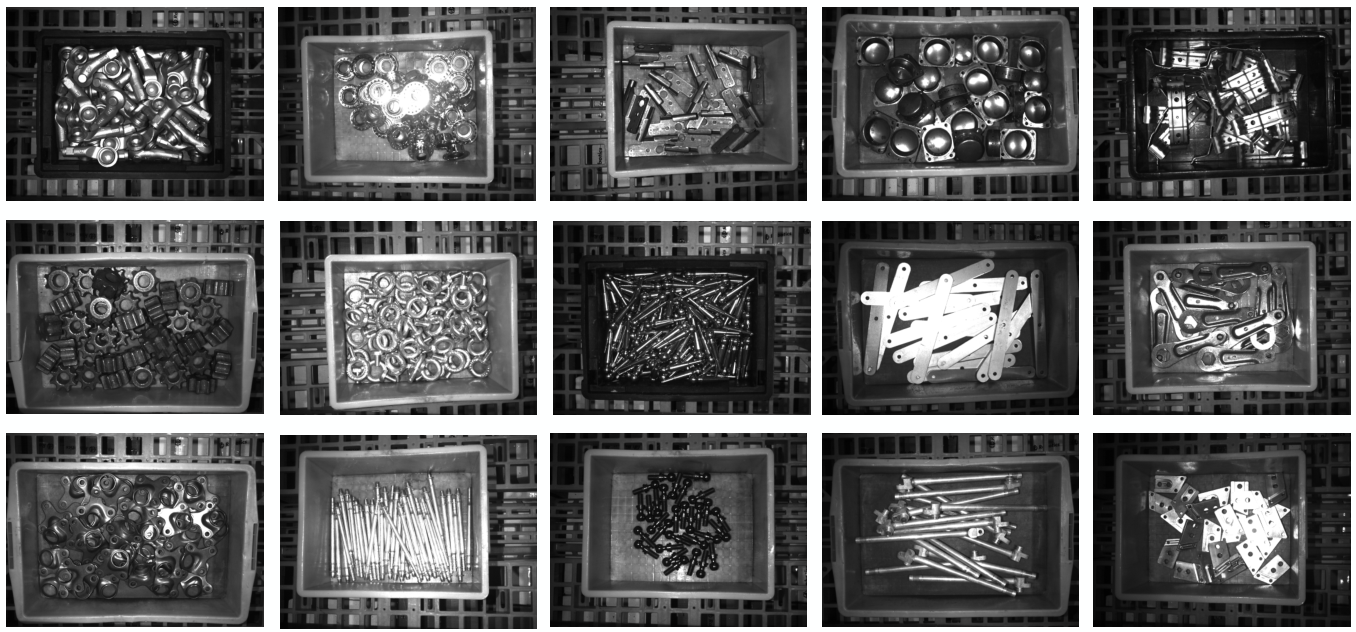
\includegraphics[width=\linewidth]{scenes.png}
\end{minipage}
\par\centering\smalltxt\textbf{Reflets, symétries et occultations}
\end{column}
\end{columns}
\par\vspace{8mm}
\centering
\textbf{15 types de pièces}\qquad \textbf{75 scènes réelles}\qquad
\textbf{$\approx$ 273\,000 annotations}
\end{frame}

% 2. Hardware : figure 5 de l'article.
\begin{frame}{Hardware}
\src{Huang et al., §3.1 et figure 5.}
\begin{columns}[c,onlytextwidth]
\begin{column}{.62\textwidth}
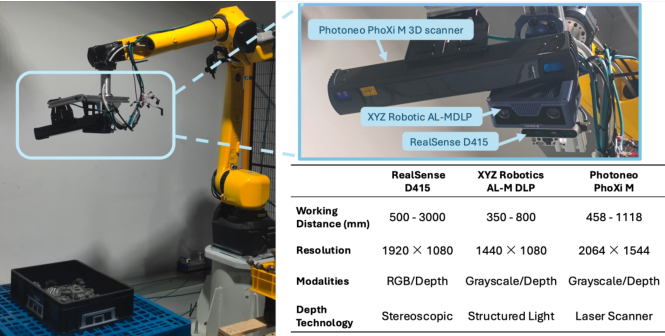
\includegraphics[width=\linewidth]{robot.png}
\end{column}
\begin{column}{.33\textwidth}
\key{Bras FANUC M10iD/8L}
\par\smalltxt Répétabilité : $\pm 0{,}06$ mm.

\par\vspace{6mm}
\key{Trois capteurs}
\par\textbf{RealSense D415}\\
Stéréovision
\par\textbf{XYZ Robotics AL-M}\\
Lumière structurée
\par\textbf{Photoneo PhoXi M}\\
Triangulation laser

\par\vspace{5mm}
\textbf{50 points de vue par scène}
\end{column}
\end{columns}
\end{frame}

% 3. Data acquisition : pipeline et effet du spray.
\begin{frame}[t]{Data acquisition pipeline}
\src{Huang et al., §3.2, figures 6 (partie supérieure) et 7.}
\centering
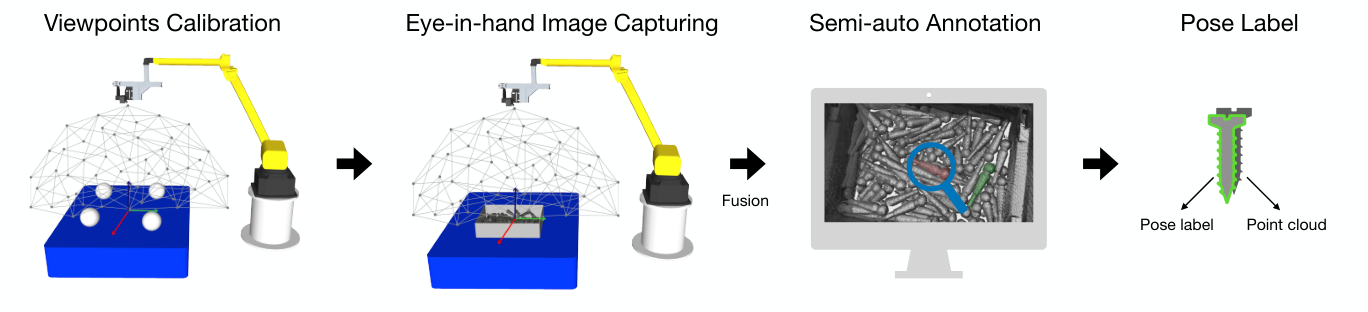
\includegraphics[width=.86\textwidth,height=45mm,keepaspectratio]{acquisition.png}
\par\vspace{3mm}
\begin{columns}[T,onlytextwidth]
\begin{column}{.43\textwidth}
\raggedright\key{Calibration}
\par\smalltxt
50 vues et 4 sphères de référence.
\par Initialisation main--œil et cinématique,\\
puis raffinement par ICP.
\par\vspace{3mm}
\textbf{RMSE : 0,248 mm}
\end{column}
\begin{column}{.53\textwidth}
\raggedright\key{Multi-pass scene capture}
\par\smalltxt
Avec antireflet : profondeur pour l'annotation.\\
Après évaporation ($\approx$ 15 min) : images natives.
\par\vspace{1mm}
\centering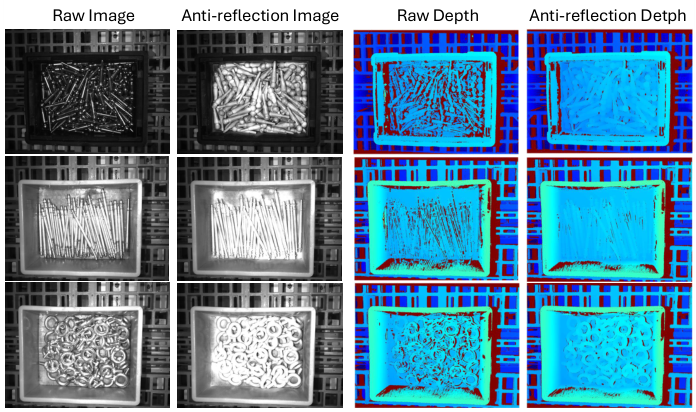
\includegraphics[width=100mm,height=57mm,keepaspectratio]{spray.png}
\end{column}
\end{columns}
\end{frame}

% 4. Validation indirecte des annotations.
\begin{frame}{Annotation error quantification}
\src{Huang et al., §3.3 et tableau 3. Résultats mesurés en simulation.}
\begin{columns}[T,onlytextwidth]
\begin{column}{.29\textwidth}
\key{1. Data noise recovery}
\end{column}
\begin{column}{.67\textwidth}
\(\displaystyle D_{\mathrm{bruité}}=D_{\mathrm{exact}}+\varepsilon,\qquad
\varepsilon\sim\mathcal N(0,\sigma^2)\)
\par\smalltxt
\textbf{$\sigma=0{,}26$ mm} pour retrouver la RMSE réelle de \textbf{0,248 mm}.
\end{column}
\end{columns}
\lightline
\begin{columns}[T,onlytextwidth]
\begin{column}{.29\textwidth}
\key{2. Même pipeline}
\end{column}
\begin{column}{.67\textwidth}
Scènes simulées : fusion multi-vues, annotation manuelle et ICP.
\par\smalltxt
Appariement hongrois avec les poses exactes.
\end{column}
\end{columns}
\lightline
\begin{columns}[T,onlytextwidth]
\begin{column}{.29\textwidth}
\key{3. Résultats}
\par\smalltxt Erreurs moyennes
\end{column}
\begin{column}{.30\textwidth}
\bignum{0,999 mm}
\par\smalltxt Position\qquad ($\sigma=0{,}12$ mm)
\end{column}
\begin{column}{.32\textwidth}
\bignum{0,432$^\circ$}
\par\smalltxt Orientation\qquad ($\sigma=0{,}08^\circ$)
\end{column}
\end{columns}
\par\vspace{5mm}
{\captiontxt\color{muted}Une moyenne en simulation ne garantit pas une erreur $<1$ mm sur chaque annotation réelle.}
\end{frame}

% 5. Les quatre tâches sont le croisement des deux lignes et des deux colonnes.
\begin{frame}{Benchmark : données et tâches}
\src{Huang et al., §4.1--4.2. Les scènes de validation et de test sont distinctes.}
\begin{columns}[T,onlytextwidth]
\begin{column}{.49\textwidth}
\key{Répartition du dataset}
\par\vspace{4mm}
{\smalltxt
\renewcommand{\arraystretch}{1.65}
\begin{tabularx}{\linewidth}{@{}lXr@{}}
\toprule
\textbf{Ensemble} & \textbf{Données} & \textbf{Images}\\
\midrule
Entraînement & Synthétiques & 45\,000\\
Validation & 15 scènes réelles & 2\,250\\
Test & 60 scènes réelles & 9\,000\\
\bottomrule
\end{tabularx}}
\end{column}
\begin{column}{.45\textwidth}
\key{Quatre tâches}
\par\vspace{4mm}
{\smalltxt
\renewcommand{\arraystretch}{1.65}
\begin{tabularx}{\linewidth}{@{}Xcc@{}}
\toprule
 & \textbf{Seen} & \textbf{Unseen}\\
\midrule
Détection 2D & $\checkmark$ & $\checkmark$\\
Pose 6D & $\checkmark$ & $\checkmark$\\
\bottomrule
\end{tabularx}
\par\vspace{4mm}
\textbf{Seen :} entraînement sur les objets du dataset.
\par\textbf{Unseen :} aucun réentraînement sur ces objets.}
\end{column}
\end{columns}
\par\vspace{8mm}
\textbf{Les modèles CAO sont disponibles dans les quatre tâches.}
\end{frame}

% 6. Conventions BOP : une symétrie globale pour l'ensemble du modèle.
% Référence : Hodaň et al., BOP Challenge 2020, §2.2, équations (2)--(3).
% https://arxiv.org/abs/2009.07378
% https://github.com/thodan/bop_toolkit/blob/master/bop_toolkit/pose_error.py
\begin{frame}{Critères d'évaluation}
\src{Huang et al., §4.3. Formules selon BOP : $\min_S\max_x$ (ordre inversé dans les formules imprimées de l'article).}
\begin{columns}[T,onlytextwidth]
\begin{column}{.33\textwidth}
\key{Détection 2D}
\par\vspace{4mm}
\[
\operatorname{IoU}(\widehat M,M)
=\frac{|\widehat M\cap M|}{|\widehat M\cup M|}
\]
\par\vspace{4mm}
\smalltxt
\textbf{AP :} score issu de la courbe précision--rappel.
\par\vspace{3mm}
Moyenne sur les seuils IoU
\[
\tau\in\{0{,}50;\,0{,}55;\,\ldots;\,0{,}95\}
\]
et sur les catégories.
\end{column}
\begin{column}{.63\textwidth}
\key{Pose 6D}
\par\vspace{4mm}
\textbf{MSSD}\quad{\smalltxt Distance 3D, en mm}
\[
e_{\mathrm{MSSD}}
=\min_{S\in\mathcal S}\;\max_{x\in\mathcal M}\,
\bigl\|\widehat T x-T_{\mathrm{GT}}Sx\bigr\|_2
\]
\par\vspace{2mm}
\textbf{MSPD}\quad{\smalltxt Distance de reprojection, en pixels}
\[
e_{\mathrm{MSPD}}
=\min_{S\in\mathcal S}\;\max_{x\in\mathcal M}\,
\bigl\|\Pi(\widehat T x)-\Pi(T_{\mathrm{GT}}Sx)\bigr\|_2
\]
{\captiontxt $\mathcal M$ : points CAO ; $\mathcal S$ : symétries ; $\Pi$ : projection caméra.}
\par\vspace{3mm}
\smalltxt
Pose correcte si $e<\theta$.\\
AP moyennée sur les seuils, les objets et les deux métriques.
\end{column}
\end{columns}
\end{frame}

% 7. Sélection compacte du tableau 4.
\begin{frame}{Résultats et conclusion}
\src{Huang et al., sélection du tableau 4 et §4.4--4.5. BOP-Core 5 : moyenne des cinq datasets comparés.}
\centering
{\smalltxt
\renewcommand{\arraystretch}{1.6}
\begin{tabularx}{.94\textwidth}{@{}lXlrr@{}}
\toprule
\textbf{Tâche} & \textbf{Méthode} & \textbf{Régime} &
\textbf{AP BOP-Core 5} & \textbf{AP XYZ-IBD}\\
\midrule
2D & YOLOX & Seen & 0,798 & \textbf{0,774}\\
2D & SAM-6D & Unseen & 0,449 & \textbf{0,296}\\
\midrule
6D & GDRNet & Seen & 0,827 & \textbf{0,266}\\
6D & SAM-6D & Unseen & 0,704 & \textbf{0,578}\\
\bottomrule
\end{tabularx}}
\par\vspace{5mm}
\raggedright
\begin{itemize}\setlength\itemsep{3mm}
\item \textbf{2D :} YOLOX reste stable, les méthodes unseen reculent.
\item \textbf{6D :} forte baisse des méthodes seen, scores mieux préservés en unseen.
\end{itemize}
\par\vspace{4mm}
\key{Les scènes industrielles restent difficiles pour les méthodes évaluées.}
\par\vspace{2mm}
{\captiontxt\color{muted}Comparaison de chaînes complètes : détecteurs, architectures et préentraînements différents.}
\end{frame}

\end{document}
